\documentclass{article}
\usepackage{pgfplots}
\usetikzlibrary{math}
\pgfplotsset{compat=1.16}
\usepackage{xfp}

\begin{document}

Intervalo de confianza para la media, si la media muestral es:6.32, la desviación típica: 2.3, tamaño de la muestra: 100 y el grado de confianza: 95.0\%. \\ \\ 
$\alpha=1-0.95=0.05\to \frac{\alpha}{2}=0.025$ \\ \\ Valor crítico: \\ $P(Z>z_{\alpha/2})=0.025\to P(Z<z_{\alpha/2})=0.975 \to z_{\alpha/2} =1.96$ \\ 
  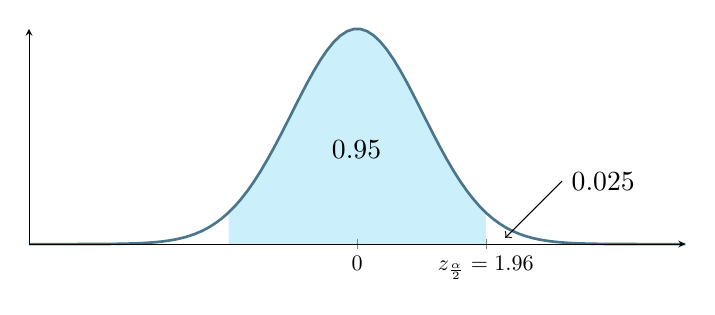
\begin{tikzpicture}[scale=0.8]
    \pgfmathdeclarefunction{gauss}{2}{\pgfmathparse{1/(#2*sqrt(2*pi))*exp(-((x-#1)^2)/(2*#2^2))}}
    \tikzmath{\conf = 0.95; \crit= 1.96; \a=0.025);}
    \begin{axis}[no markers, domain=-5:5, samples=100, axis lines=left, height=5cm, width=12cm, xtick={0,\crit}, ytick=\empty, xticklabels = {$0$, $z_{\frac{\alpha}{2}}=\crit$},enlargelimits=false, clip=false, axis on top]
      \addplot [fill=cyan!20, draw=none, domain=-\crit:\crit] {gauss(0,1)} \closedcycle;
      \addplot [very thick,cyan!50!black] {gauss(0,1)};
    \end{axis}
    \node[] at (5.2,1.5) {$\conf$};	
    \draw[->]   (\crit+6.5,1)node[right]{$\a$}  --  (\crit+5.6,0.1) ;
  \end{tikzpicture} \\
  Error cometido: \\ $E=z_{\alpha/2}\cdot \frac{\sigma}{\sqrt{n}} \to E=1.96\cdot \frac{2.3}{10.0}=0.4508$ \\ Por tanto el intervalo de confianza será: \\$\left(\overline{x} - E , \overline{x} + E \right)=\left(6.32 - 0.4508 , 6.32 + 0.4508 \right)=\left(5.8692, 6.7708 \right)$ \\  \\ 
  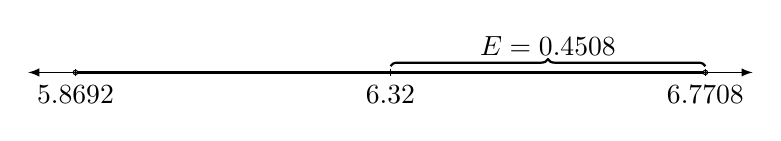
\begin{tikzpicture}[scale=0.4]
      \tikzmath{\a = -10; \b = 10; \aa = \a -1; \bb = \b + 1 ; \dist = \b - \a; \med = (\a + \b)/2;}
      \draw[very thick] (\a,0) -- (\b,0);
      \path [draw=black, fill=white] (\b,0) circle (2pt);
      \path [draw=black, fill=white] (\a,0.0) circle (2pt);
      \draw[latex-latex] (\a - 1.5,0) -- (\b + 1.5,0) ;
      \draw[shift={(\a,0)},color=black] (0pt,3pt) -- (0pt,-3pt);
      \draw[shift={(\a,0)},color=black] (0pt,0pt) -- (0pt,-3pt) node[below] {$5.8692$};
      \draw[shift={(\med,0)},color=black] (0pt,3pt) -- (0pt,-3pt);
      \draw[shift={(\med,0)},color=black] (0pt,0pt) -- (0pt,-3pt) node[below] {$6.32$};
      \draw[shift={(\b,0)},color=black] (0pt,3pt) -- (0pt,-3pt);
      \draw[shift={(\b,0)},color=black] (0pt,0pt) -- (0pt,-3pt) node[below] {$6.7708$};
      \draw[decorate,decoration={brace}, thick](\med,0.2)--(\b,0.2) node[above, midway] {$E=0.4508$}; 
  \end{tikzpicture} \\
  
  
  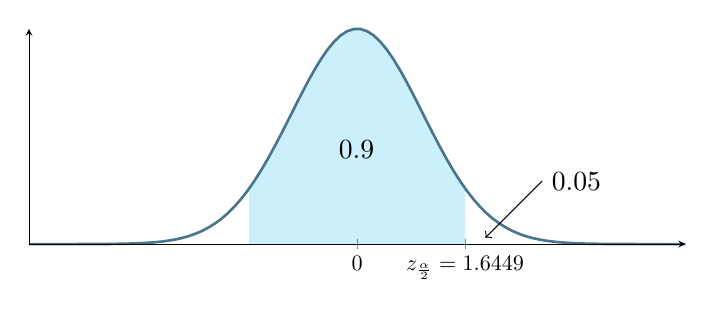
\begin{tikzpicture}[scale=0.8]
    \pgfmathdeclarefunction{gauss}{2}{\pgfmathparse{1/(#2*sqrt(2*pi))*exp(-((x-#1)^2)/(2*#2^2))}}
    \tikzmath{\conf = 0.9; \crit= 1.6449; \a=0.05);}
    \begin{axis}[no markers, domain=-5:5, samples=100, axis lines=left, height=5cm, width=12cm, xtick={0,\crit}, ytick=\empty, xticklabels = {$0$, $z_{\frac{\alpha}{2}}=\crit$},enlargelimits=false, clip=false, axis on top]
      \addplot [fill=cyan!20, draw=none, domain=-\crit:\crit] {gauss(0,1)} \closedcycle;
      \addplot [very thick,cyan!50!black] {gauss(0,1)};
    \end{axis}
    \node[] at (5.2,1.5) {$\conf$};	
    \draw[->]   (\crit+6.5,1)node[right]{$\a$}  --  (\crit+5.6,0.1) ;
  \end{tikzpicture} 
\end{document}